WebSocketのプロトコルは実に簡単です。はじめのhandshakeが通った後、接続の確立に成功します。この後のデータの通信はすべて"\textbackslash x00"から始まり、"\textbackslash xFF"で終わります。クライアントではこれは透明です。WebSocketモジュールは自動的にオリジナルのデータから大事なところを残してあとは取り除いてくれます。

ブラウザがWebSocketの接続リクエストを送信すると、サーバはレスポンスを送信します。その後接続の確立に成功します。この過程を通常"ハンドシェイク"(handshaking)と呼びます。下のリクエストとフィードバック情報をご覧ください:

\begin{figure}[H]
  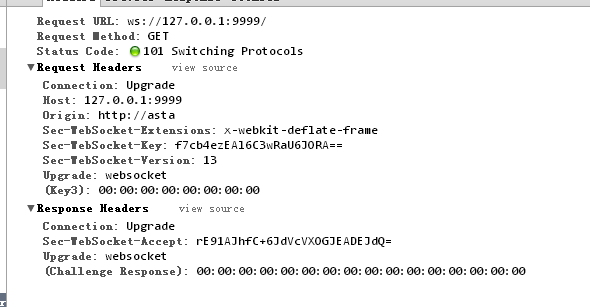
\includegraphics[width=14cm]{8.2.websocket2.png}
  \label{図8.3}
   \caption{WebSocketのrequestとresponse情報}
\end{figure}

リクエストの"Sec-WebSocket-Key"はランダムです。日々エンコーディングとやりあっているプログラマにはひと目で分かります:これはbase64エンコードが施されたデータで、サーバはこのリクエストを受け取った後この文字列を固定の文字列に連結させる必要があります:


\begin{lstlisting}[numbers=none]
258EAFA5-E914-47DA-95CA-C5AB0DC85B11
\end{lstlisting}

すなわち、\texttt{f7cb4ezEAl6C3wRaU6JORA==}を上の固定の文字列に連結し、このような文字列を生成します:

\begin{lstlisting}[numbers=none]
f7cb4ezEAl6C3wRaU6JORA==258EAFA5-E914-47DA-95CA-C5AB0DC85B11
\end{lstlisting}

この文字列に対しまずsha1セキュリティハッシュアルゴリズムを使って2進数の値を計算します。その後base64を使ってこれをエンコードし、ハンドシェイク後の文字列を得ることができます:



\begin{lstlisting}[numbers=none]
rE91AJhfC+6JdVcVXOGJEADEJdQ=
\end{lstlisting}

これをレスポンスヘッダ\texttt{Sec-WebSocket-Accept}の値としてクライアントに返します。



